\documentclass{article}
\usepackage{graphicx} % Required for inserting images
\usepackage{amsmath}
\usepackage{float}
\usepackage{siunitx}
\usepackage{caption}
\usepackage{subcaption}
\usepackage{hyperref}


\title{PHY 338k Lab Report 2}
\author{Lily Nguyen with Anna Grove}
\date{October 7, 2025}

\begin{document}

\maketitle

\section{Lab 4: Diode Circuits}

\subsection{Oscilloscope probe}

\subsubsection{Compensation capacitor}

To obtain accurate waveform measurements, we must ensure the oscilloscope probe
is properly compensated so that its RC time constant matches the oscilloscope
input. We connected the probe to the scope's Probe Comp terminal and adjusted
the small screw near the probe connector while observing the waveform.
Figure~\ref{fig:compensation_all} shows the three compensation states.

\begin{enumerate}
    \item When \textbf{under-compensated}, the square wave has rounded edges
    because the probe capacitance is too small, limiting high-frequency response.
    \item When \textbf{over-compensated}, the waveform overshoots at transitions
    since the probe capacitance is too large, which over-emphasizes higher
    frequency components.
    \item When \textbf{properly compensated}, the waveform displays flat tops
    and sharp corners, indicating a balanced frequency response.
\end{enumerate}

\noindent These changes occur because a square wave contains many harmonics,
so any mismatch between the probe and scope capacitances would cause unequal
attenuation of those harmonics and distort the waveform. Thus, proper adjustment
ensures that the measured signal accurately represents the true voltage at the
circuit node.

\begin{figure}[H]
    \centering
    \begin{subfigure}[t]{0.32\textwidth}
        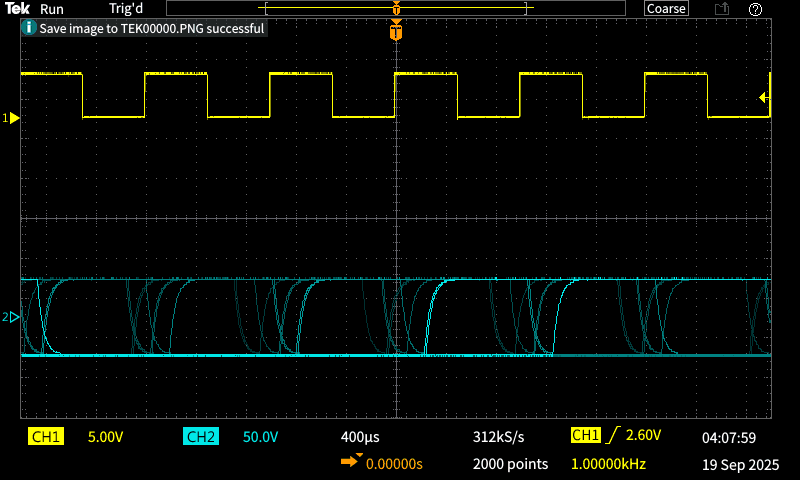
\includegraphics[width=\linewidth]{4.1a.full.png}
        \caption{Properly Compensated}
        \label{fig:full}
    \end{subfigure}
    \hfill
    \begin{subfigure}[t]{0.32\textwidth}
        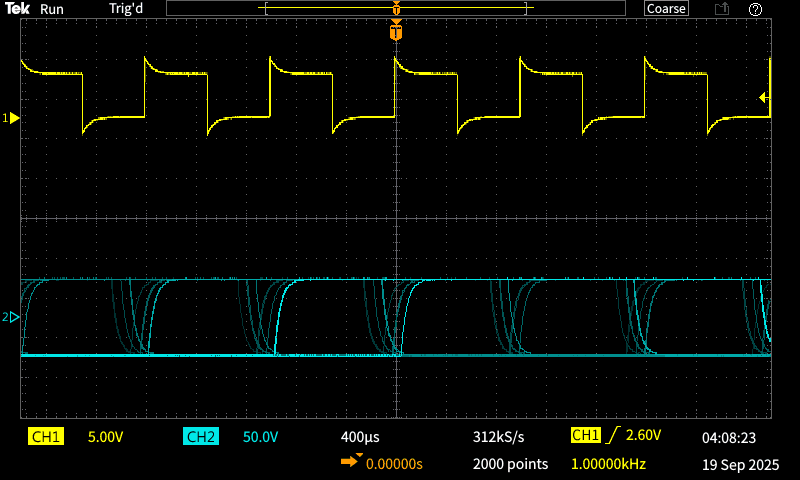
\includegraphics[width=\linewidth]{4.1a.side1.png}
        \caption{Over-compensated}
        \label{fig:over}
    \end{subfigure}
    \hfill
    \begin{subfigure}[t]{0.32\textwidth}
        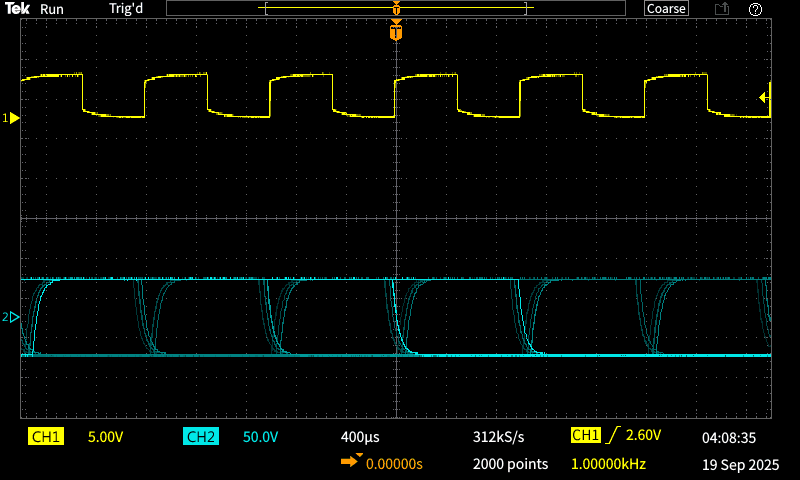
\includegraphics[width=\linewidth]{4.1a.side2.png}
        \caption{Under-compensated}
        \label{fig:under}
    \end{subfigure}
    \caption{Oscilloscope traces for different probe compensation settings. 
    Proper compensation yields flat tops and clean edges, whereas incorrect 
    compensation leads to overshoot or rounding.}
    \label{fig:compensation_all}
\end{figure}


\subsubsection{Reduction of oscilloscope load on a signal with a 10x probe}

We used two configurations to explore the effects of oscilloscope loading in
this section. Circuit A used a direct BNC connection from the function generator
to CH2 and Circuit B used a 10x probe connection to CH2. In both cases, we
connected CH1 to the generator output as a reference.\\

\noindent At low frequencies, both configurations produced similar waveforms. As we
increased the frequency, the we observed reduced amplitude and distortion in
Circuit A's scope display due to the oscilloscope's finite input impedance and
capacitance. At $f=3.0\si{\kilo\hertz}$, we measured an amplitude ratio of:

\begin{equation}
    \frac{V_{\text{CH2}}}{V_{\text{CH1}}}=\frac{8.8\si{\volt}}{15.2\si{\volt}}=0.58.
\end{equation}

\noindent When we added the 10x probe, the measured CH2 amplitude increased to $13.8\si{\volt}$,
giving an amplitude ratio of:
\begin{equation}
    \frac{V_{\text{CH2}}}{V_{\text{CH1}}}=\frac{13.8\si{\volt}}{15.2\si{\volt}}=0.91.
\end{equation}

\noindent Furthermore, the waveform closely matched CH1 with negligible phase
shift. Our results agree well with the theoretical predictions from Homework 2,
where the 10x probe's higher input impedance and reduced capacitance were
expected to minimize loading.

\begin{figure}[H]
    \centering
    \begin{subfigure}[t]{0.48\textwidth}
        \centering
        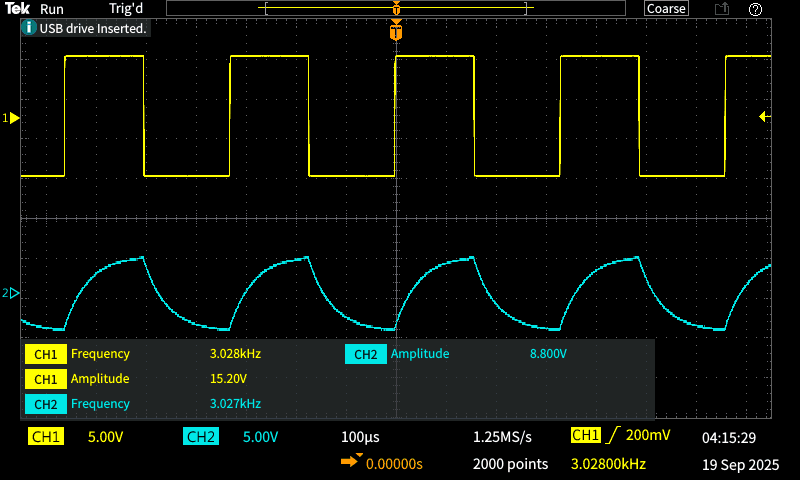
\includegraphics[width=\linewidth]{4.1b.A.png}
        \caption{Direct scope connection (Circuit A): significant distortion and reduced amplitude.}
        \label{fig:circuit_a}
    \end{subfigure}
    \hfill
    \begin{subfigure}[t]{0.48\textwidth}
        \centering
        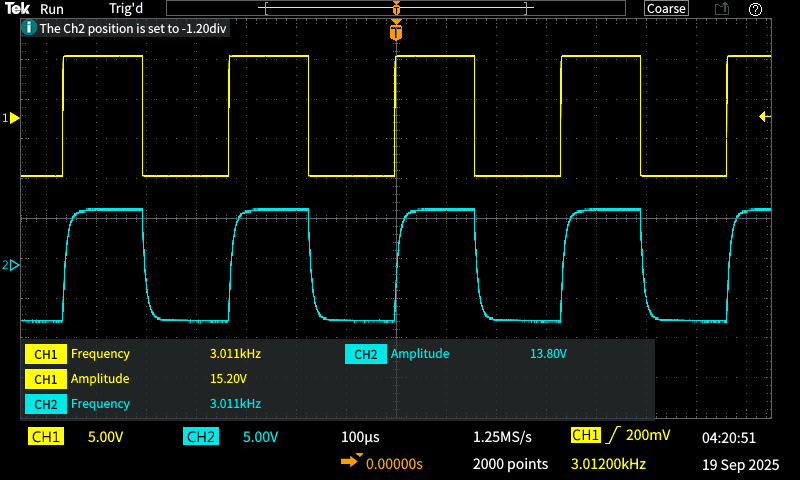
\includegraphics[width=\linewidth]{4.1b.B.png}
        \caption{10x probe connection (Circuit B): restored amplitude and cleaner waveform.}
        \label{fig:circuit_b}
    \end{subfigure}
    \caption{Scope displays showing the effect of oscilloscope loading with and without a 10x probe at \SI{3.0}{\kilo\hertz}.}
    \label{fig:circuits_ab}
\end{figure}

\noindent Thus, we confirm the 10x probe minimizes loading by preserving both
amplitude and waveform integrity, making it essential for accurate measurements
in high-impedance or high-frequency circuits.

\subsection{Diode circuits}

\subsubsection{Multimeter diode test}

Using the diode test mode on the digital multimeter, we measured to the forward
voltage of the 1N4007 diode to be $0.562\si{\volt}$ and the reverse voltage to 
be $3.122\si{\volt}$. The forward reading indicates a typical silicon diode drop
of approximately $0.6\si{\volt}$, whereas the reverse reading reflects the
multimeter's open-circuit voltage, indicating that negligible current flows when
the diode is reverse-biased. Our measurements validate that the 1N4007 conducts in
the forward direction and effectively blocks current in the reverse direction, so
we confirm our device functions as expected.


\subsubsection{Half-wave rectifier}

We constructed a half-wave rectifier using a 1N4007 diode and a $4\si{\volt}$
amplitude, and a $1.021\si{\kilo\hertz}$ input sine wave. The measured waveforms for
$V_{\text{in}}$ and $V_{\text{out}}$ (CH2) are shown in Figure~\ref{fig:half_wave}.\\

\noindent At $1.02\si{\kilo\hertz}$, $V_{\text{in}}$ ranged from $3.9\si{\volt}$ to 
$-4.5\si{\volt}$, while $V_{\text{out}}$ varied from $29.6\si{\volt}$ to $-0.80\si{\volt}$. 
The apparent voltage amplification is due to probe scaling rather than
actual circuit gain. Qualitatively, the output waveform displays the expected
half-wave rectifier behavior where current flows only during the positive 
half-cycles when the diode is forward-biased and is blocked during the negative
half-cycles.\\

\begin{figure}[H]
    \centering
    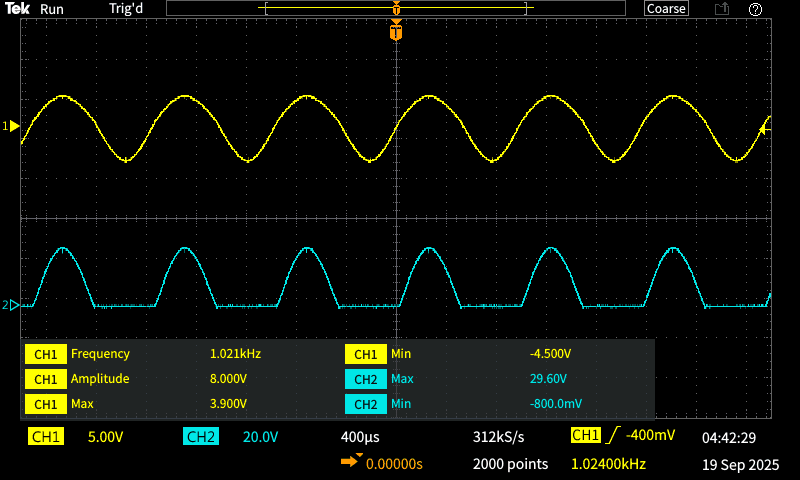
\includegraphics[width=0.65\linewidth]{4.2.b.png}
    \caption{Input (CH1) and output (CH2) waveforms for the half-wave rectifier at $1\si{\kilo\hertz}$.}
    \label{fig:half_wave}
\end{figure}

\noindent The maximum output voltage $V_{2(\text{max})}$ occurs when the diode conducts 
on the positive half-cycle. It's slightly lower than the input peak because of the
diode's forward voltage drop ($V_{\text{drop}}\approx0.7\si{\volt}$), so 
$V_{2(\text{max})}\approx V_{\text{in, peak}}-V_{\text{drop}}\approx 3.2\si{\volt}$.
Our measured value differs due to the oscilloscope scaling factor. The minimum
output voltage $V_{2(\text{min})}$ occurs where the diode is reverse-biased since
the current is blocked, ideally producing $0\si{\volt}$ across the load.\\

\noindent Thus, our observed waveform confirms the expected behavior of a half-wave rectifier
where positive cycles exhibit conduction and negative cycles exhibit suppression,
yielding a pulsating DC output.


\subsubsection{Diode clamp}

We tested a diode clamp circuit using a $10\si{\volt}$ amplitude and $1\si{\kilo\hertz}$
sine wave. Our goal with this circuit was to shift the input waveform upward and fix its
negative peaks near $+5\si{\volt}$ to produce a pulsing DC output. The input ($V_{\text{in}}$) and output ($V_{\text{out}}$) waveforms are displayed
in Figure~\ref{fig:diode_clamp}.\\

\noindent At $1.079\si{\kilo\hertz}$, the $V_{\text{in}}$ ranged from $12.5\si{\volt}$ to $-10.3\si{\volt}$,
while $V_{\text{out}}$ ranged from $58.0\si{\volt}$ to $-104.0\si{\volt}$ as
displayed on the oscilloscope. The apparent voltage difference is due to probe
scaling rather than actual gain. We observed a flattened peaks instead of the
expected uniform shift in the output waveform, which suggests that our circuit
behaved more like a diode clipper than a true clamp.

\begin{figure}[H]
    \centering
    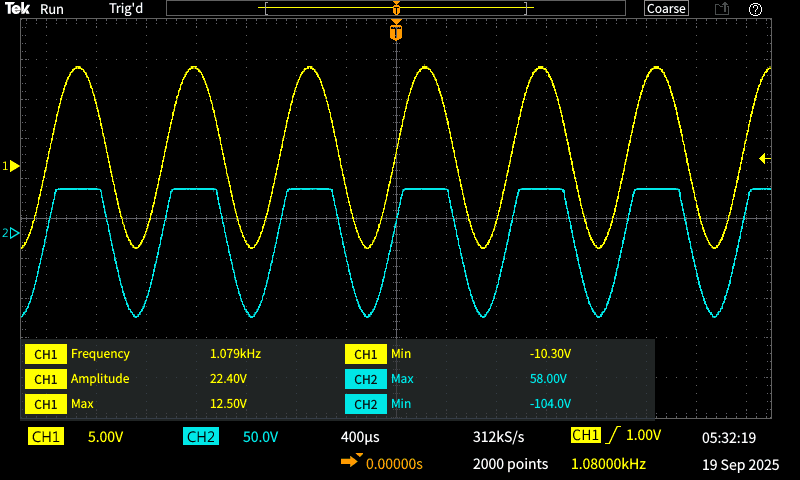
\includegraphics[width=0.65\linewidth]{4.2.e.png}
    \caption{Input (CH1) and output (CH2) waveforms for the diode clamp circuit at $1\si{\kilo\hertz}$.}
    \label{fig:diode_clamp}
\end{figure}

\noindent In theory, a diode clamp would shift the DC reference of an AC waveform without
altering its shape. During the negative half-cycle, the diode conducts and charges
the capacitor to the input's peak value. When the signal swings positive, the diode
becomes reverse-biased, and the stored charge acts as a DC offset that raises
the entire waveform and clamps its minimum voltage near $+5\si{\volt}$.\\

\noindent In our experiment, the clipping behavior we observed suggests that
the capacitor did not charge properly or that the bias connection was incorrect.
As a result, the diode limited the voltage supply rather than shifting the
waveform baseline. Despite this possible mistake, our data still shows the
diode's rectifying action and voltage-limiting effect, which is consistent with
partial conduction near the $+5\si{\volt}$ bias.


\subsubsection{Zener diode IV curve}

Finally, we measured the current vs. reverse voltage for the 1N4736 Zener diode
with the TTi EL302R power supply in reverse-bias configuration. Our measurements
are shown in Table~\ref{tab:zener_table}, and the corresponding IV-curve is 
plotted in Figure~\ref{fig:zener}.

\begin{figure}[H]
    \centering
    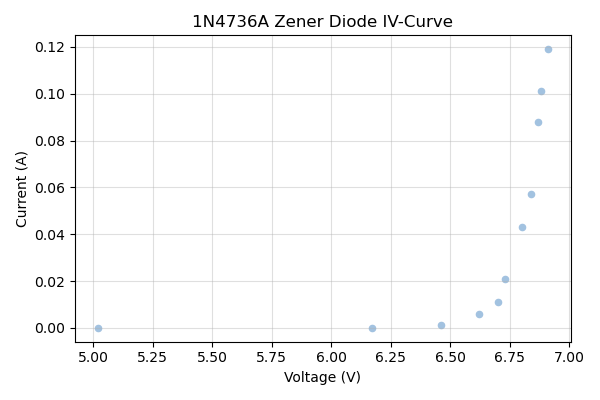
\includegraphics[width=0.6\linewidth]{4.2eplot.png}
    \caption{IV plot for the 1N4736A Zener diode.}
    \label{fig:zener}
\end{figure}

\begin{table}[H]
\centering
    \begin{tabular}{|c|c|}
    \hline
    Voltage (V) & Current (mA) \\
    \hline
    5.02 & 0.022 \\
    6.17 & 0.097 \\
    6.46 & 1.25 \\
    6.62 & 5.80 \\
    6.70 & 10.9 \\
    6.73 & 20.7 \\
    6.80 & 43.0 \\
    6.84 & 57.0 \\
    6.87 & 88.0 \\
    6.88 & 101.0 \\
    6.91 & 119.0 \\
    \hline
    \end{tabular}
    \caption{Measured reverse current as a function of voltage for the 1N4736A Zener diode.
    Most data points were taken near the breakdown region ($6.5$-$9.6\si{\volt})$,
    where the current rises from $1\si{\milli\ampere}$ to $120\si{\milli\ampere}$
    while the voltage remains nearly constant.}
    \label{tab:zener_table}
\end{table}

\noindent At low reverse voltages (below approximately $6.3\si{\volt}$), we
observed only small leakage current in the $\si{\micro\ampere}$ range. Once we
reached the reverse voltage $V_\text{reverse}\approx6.6\si{\volt}$, the current
increased rapidly for small changes in voltage. Between $50\si{\milli\ampere}$
and $100\si{\milli\ampere}$, the voltage remained nearly constant around
$6.8\si{\volt}$, which confirms the zener diode's voltage regulation behavior. Thus,
we confirm that the diode maintains a stable output voltage despite significant changes
in current, a property that is useful for voltage reference and regulation circuits.



\section{Lab 5: Bipolar Junction Transistors}

\subsection{Multimeter Measurements}

\subsubsection{Measurements using diode test function}

We used the diode test mode of a digital multimeter to investigate the
junction behavior of three bipolar junction transistors: the 2N3904, 2N2222, and
2N3906. For each device, we measured the voltage drops between the emitter,
base, and collector terminals in both polarities to simulate diode junctions as
shown in the equivalent circuit model.\\

\noindent The table below summarizes our measured voltage drops:

\begin{table}[H]
  \centering
  \begin{tabular}{|l|c|c|c|}
    \hline
    Measurement & 2N3904 (NPN) & 2N2222 (NPN) & 2N3906 (PNP) \\
    \hline
    $V_{E \rightarrow B}$ (E more +) & 3.190 V & 3.189 V & 0.705 V \\
    $V_{B \rightarrow E}$ (B more +) & 0.717 V & 0.671 V & 3.189 V \\
    $V_{C \rightarrow B}$ (C more +) & 3.189 V & 3.189 V & 0.696 V \\
    $V_{B \rightarrow C}$ (B more +) & 0.714 V & 0.656 V & 3.189 V \\
    \hline
  \end{tabular}
  \caption{Diode voltage drops measured with DMM for three BJT types.}
\end{table}

\noindent For the NPN transistors (2N3904 and 2N2222), the base-emitter and base-collector
junctions behave like forward-biased diodes when the base is more positive, with
typical voltage drops around 0.6 to 0.7 V. When we reversed the polarity, the
measured voltages are much higher, which is consistent with reverse-biased junctions.\\

\noindent For the PNP transistor (2N3906), we observed the opposite behavior. The emitter-base and
collector-base junctions conducted when the emitter or collector was more
positive than the base, with forward voltage drops around 0.7 V.\\

\noindent Our results are consistent with the expected behavior of BJTs and allow us to 
distinguish between the NPN and PNP types based on polarity and voltage drop direction.

\subsubsection{Measurements using transistor $h_{FE}$ measurement}

Next, we measured the DC current gain $h_{FE}$ of each transistor using the DMM’s 
transistor gain function. The results are shown in the table below:

\begin{table}[H]
    \centering
    \begin{tabular}{|c|c|}
        \hline
        Transistor & $h_{FE}$ \\
        \hline
        2N3904 & 297 \\
        2N2222 & 208 \\
        2N3906 & 305 \\
        \hline
    \end{tabular}
    \caption{Measured current gain \( h_{FE} \) for each transistor.}
\end{table}

\subsection{Basic transistor circuit}

\subsubsection{$I_c$ vs. $V_{CE}$ at fixed $V_{in}$}

We investigated the behavior of a 2N2222 NPN BJT by measuring the collector-emitter
voltage $V_{CE}$ for a fixed $V_{in}$ shown in Figure~\ref{fig:ic_vs_vce}.
The curve shows a rapid increase in $I_C$ at low $V_{CE}$, followed by a
plateau region where $I_C$ remains approximately constant despite further
increases in $V_{CE}$. The flat region corresponds to the active mode of the
transistor where it behaves like a current source.

\begin{figure}[H]
    \centering
    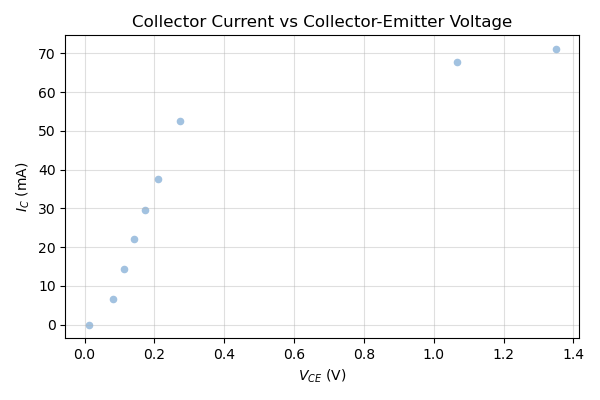
\includegraphics[width=0.75\linewidth]{5.2a.png}
    \caption{Plot of $I_C$ vs. $V_{CE}$ for fixed $V_{in}$.}
    \label{fig:ic_vs_vce}
\end{figure}

\noindent We also computed the current gain $h_{FE}=I_C / I_B$ and plotted it
against $V_{CE}$ in Figure~\ref{fig:hfe_vs_vce}. The gain increases fairly
quickly at low $V_{CE}$, then stabilizes in the active region as expected.
Across our measured points, $h_{FE}$ stabilized around 120-160, suggesting the
transistor was operating in the forward-active region.

\begin{figure}[H]
    \centering
    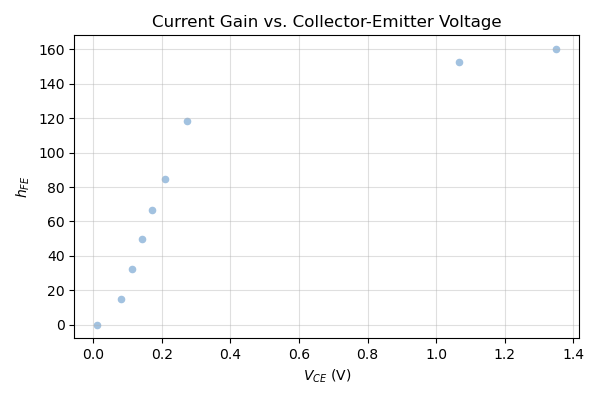
\includegraphics[width=0.75\linewidth]{5.2b.png}
    \caption{Plot of $h_{FE}$ vs. $V_{CE}$.}
    \label{fig:hfe_vs_vce}
\end{figure}

\noindent The measured gain compares reasonably well with the values listed
in the 2N2222A specifications sheet. Typical $h_{FE}$ values at $I_C=10\si{\milli\ampere}$
and $V_{CE}=10\si{\volt}$ range from 100 to 300, with a maximum of 325 for lower
collector currents. Our measured value using the DMM in the previous section was $208$, 
which also falls within the specified range, though it is slightly lower than
what we observed under circuit bias conditions.\\

\noindent The saturation collector-emitter voltage $V_{CE(\text{sat})}$ is the voltage at
which $h_{FE}=10$. Based on our data, this occured around $V_{CE}\approx0.02\si{\volt}$,
which is where $I_C\approx5\si{\milli\ampere}$ and $I_B\approx0.5\si{\milli\ampere}$,
giving us $h_{FE}\approx10$. This agrees with the typical datasheet value of
$V_{CE(\text{sat})}=0.3\si{\volt}$ at $I_C=150\si{\milli\ampere}$ and $I_B=15\si{\milli\ampere}$.
Given our lower collector current value, it is expected that our saturation
voltage would be lower than the datasheet's high-current test condition.\\

\noindent Overall, our measurements confirm the expected operating characteristics of the
2N2222A and are consistent with both the theory of BJT operation and the
manufacturer specifications.

\subsubsection{$I_C$ vs. $V_{BE}$ at fixed $V_{CC}$}

To investigate the exponential relationship between base-emitter voltage $V_{BE}$
and collector current $I_C$, we set $V_{CC} = 5.0\si{\volt}$ and varied the input
voltage to sweep $I_C$ over a range from about $0.1\si{\milli\ampere}$ to
$100\si{\milli\ampere}$. We recorded both $I_C$ and $V_{BE}$ for each setting.\\

\noindent We plotted $V_{BE}$ against $I_C$ with $I_C$ on a logarithmic scale, as seen
in Figure~\ref{fig:vbe_vs_ic}. According to the Ebers-Moll relation:

\begin{equation}
I_C = I_S e^{V_{BE}/V_T},
\end{equation}

\noindent taking the natural logarithm of both sides gives us:

\begin{equation}
\ln(I_C) = \frac{V_{BE}}{V_T} + \ln(I_S).
\end{equation}

\noindent This relation predicts that a plot of $V_{BE}$ vs. $\ln(I_C)$ should yield a straight line,
assuming $I_S$ and $V_T$ are constant.

\begin{figure}[H]
    \centering
    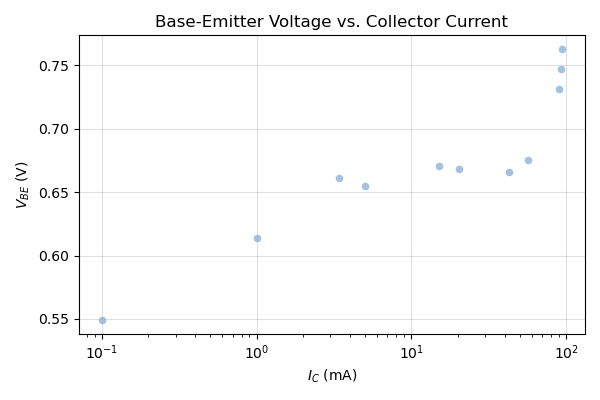
\includegraphics[width=0.75\linewidth]{5.2c.png}
    \caption{Plot of $V_{BE}$ vs. $I_C$ (log scale) at fixed $V_{CC} = 5.0\,\si{\volt}$.}
    \label{fig:vbe_vs_ic}
\end{figure}

\noindent As seen in the figure, the curve follows a roughly linear trend over the central
range of $I_C$ values, which supports the exponential dependence predicted by
the Ebers-Moll model. At higher values of $I_C$, the curve deviates from the semilog
relationship likely due to the effects of base-emitter series resistance, which are
which are not accounted for in the ideal Ebers-Moll model. These factors cause an
excess voltage drop across the base and emitter terminals, which would increase the
measured $V_{BE}$ beyond the ideal exponential prediction. Thermal effects may also
have contributed slightly by altering junction properties under high power 
dissipation.\\

\noindent Overall, the measured relationship between $V_{BE}$ and $I_C$ follows the expected
exponential behavior described by the Ebers-Moll model, especially across the lowto 
mid range of collector currents. The trend we observed is also consistent with
the base-emitter characteristic shown in Figure 4 of the 2N2222A datasheet,
which validates both our measurement procedure and the theoretical model.
Thus, we can confirm that the 2N2222A exhibits typical BJT exopnential behavior
in the active region.

\subsection{Biasing a transistor}

We built the biasing circuit using a 2N3904 NPN transistor with 
resistor values shown in Table~\ref{tab:biasing_resistors}. The voltage 
measurements at the collector, base, and emitter are given in 
Table~\ref{tab:biasing_voltages}.

\begin{table}[H]
    \centering
    \begin{tabular}{|c|c|c|}
        \hline
        Component & Calculated Value & Actual Value Used \\
        \hline
        $R_1$ & 185\,k$\Omega$ & 185\,k$\Omega$ \\
        $R_2$ & 15\,k$\Omega$ & 13.8\,k$\Omega$ \\
        $R_C$ & 10\,k$\Omega$ & 9.93\,k$\Omega$ \\
        $R_E$ & 1\,k$\Omega$ & 1.08\,k$\Omega$ \\
        \hline
    \end{tabular}
    \caption{Calculated and actual resistor values used in the biasing circuit.}
    \label{tab:biasing_resistors}
\end{table}

\begin{table}[H]
    \centering
    \begin{tabular}{|c|c|}
        \hline
        Node & Measured Voltage \\
        \hline
        $V_C$ & 57.3\,mV \\
        $V_B$ & 0.625\,V \\
        $V_E$ & 34.0\,mV \\
        \hline
    \end{tabular}
    \caption{Measured voltages at transistor terminals.}
    \label{tab:biasing_voltages}
\end{table}

\noindent The base-emitter voltage $V_{BE} = V_B - V_E \approx 0.591\si{\volt}$ is 
within the expected range for forward bias. However, the collector voltage 
$V_C = 57.3\si{\milli\volt}$ is much lower than expected, suggesting that the 
transistor is operating in saturation rather than in the forward-active region. 
To shift it into the active region (typically $V_C$ between 8 to 12V), we could
modify the circuit by increasing $R_C$ to reduce collector current or increasing 
$R_2$ to decrease the base current and base bias voltage.


\subsection{Common emitter AC amplifier}

Finally, we built a common emitter amplifier circuit and measured the input
and output sine waves across a specified range of frequencies. Figure~\ref{fig:scope_trace}
shows an example oscilloscope trace where the output signal is inverted and
amplified relative to the input, as expected for this setup.

\begin{figure}[H]
    \centering
    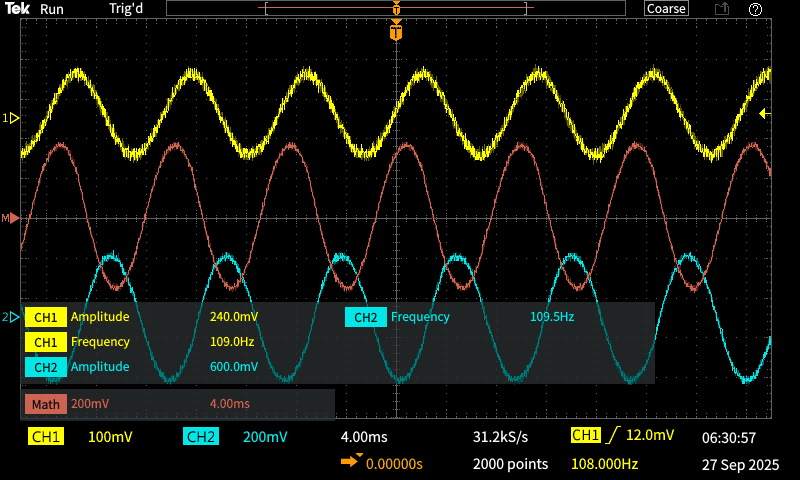
\includegraphics[width=0.7\linewidth]{5.4.3.png}
    \caption{Oscilloscope trace of input (CH1) and output (CH2) sine waves at \SI{109.0}{\hertz}.}
    \label{fig:scope_trace}
\end{figure}

\noindent To analyze frequency-dependent behavior, we calculated the voltage gain in dB
across input frequencies from $100\si{\hertz}$ to $500\si{\kilo\hertz}$. We
computed the gain as:

\begin{equation}
    \text{Voltage Gain (dB)}=20\log_{10}\left(\frac{V_{\text{out}}}{V_{\text{in}}}\right).
\end{equation}

\begin{figure}[H]
    \centering
    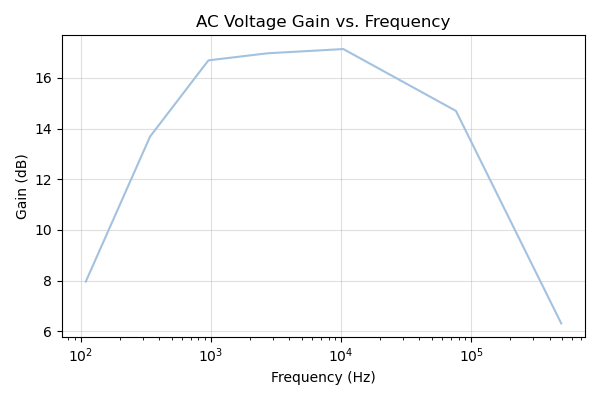
\includegraphics[width=0.7\linewidth]{5.4a.png}
    \caption{AC voltage gain vs. frequency for the common emitter amplifier.}
    \label{fig:gain_plot}
\end{figure}

\noindent The voltage gain is low at low frequencies due the high-pass filtering effect
of the coupling and emitter bypass capacitors. In the mid-frequency range, the 
gain plateaus at its maximum (approximately $17$ dB), which is where the
amplifier behaves linearly. At higher frequencies, the gain drops off, likely
due to parasistic capacitiances within the transistor and wiring, which introduce
low-pass filtering. This aligns with typical band-pass behavior for a common
emitter amplifier.



\section{Lab 6: Field Effect Transistors}

\subsection{JFET Properties}

In this section, we explored the characteristics of of the J112 n-channel JFET
and examined how the drain current responds to changes in the gate-source voltage.
We measured $I_D$ across a range of positive and negative $V_{GS}$ values and
used our results to identify the transistor's parameters as well as compare its
behavior to the J112 datasheet.\\

\noindent We plotted $I_D$ vs. $V_{GS}$ for the J112 n-channel JFET shown below.
The drain current decreases as $V_{GS}$ becomes more negative and approaches zero near 
$V_{GS} \approx -5.0\,\si{\volt}$, indicating a cutoff voltage of 
$V_{GS(\text{off})} = -5.0\,\si{\volt}$.

\begin{figure}[H]
    \centering
    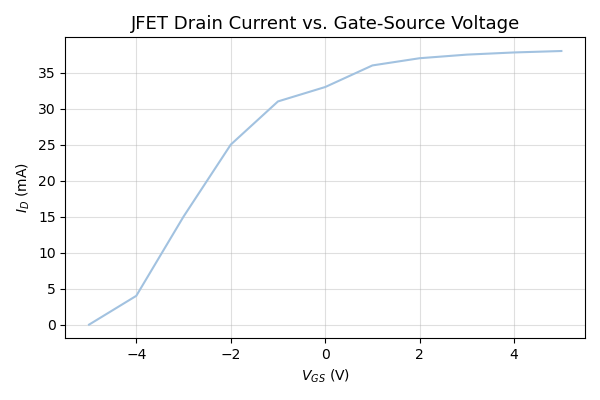
\includegraphics[width=0.8\linewidth]{6.1a.png}
    \caption{Plot of $I_D$ vs.\ $V_{GS}$ for the J112 n-channel JFET.}
    \label{fig:jfet_id_vgs}
\end{figure}

\noindent To determine the increment in gate voltage $V_{GS} - V_{GS(\text{off})}$
required to obtain a drain current of $10\,\si{\milli\ampere}$, we used the
Shockley equation:

\begin{equation}
    I_D = I_{DSS} \left( 1 - \frac{V_{GS}}{V_{GS(\text{off})}} \right)^2.
\end{equation}

\noindent Using our measured values $I_{DSS} \approx 38\,\si{\milli\ampere}$ and 
$V_{GS(\text{off})} \approx -5.0\,\si{\volt}$, we set $I_D = 10\,\si{\milli\ampere}$ 
and solved for $V_{GS}$. Our result was $V_{GS} \approx -2.44\,\si{\volt}$, which 
corresponds to an increment of:

\begin{equation}
    V_{GS} - V_{GS(\text{off})} = (-2.44) - (-5.0) = 2.56\,\si{\volt}.
\end{equation}

\noindent Thus, an increase of approximately $2.56\,\si{\volt}$ from the
cutoff voltage is required for the drain current to reach 
$10\si{\milli\ampere}$.\\

\noindent Next, we plotted $g_m$ vs. $V_{GS}$ for the J112 n-channel JFET using the equation:

\begin{equation}
    g_m = \frac{\Delta I_D}{\Delta V_{GS}}.
\end{equation}

\begin{figure}[H]
    \centering
    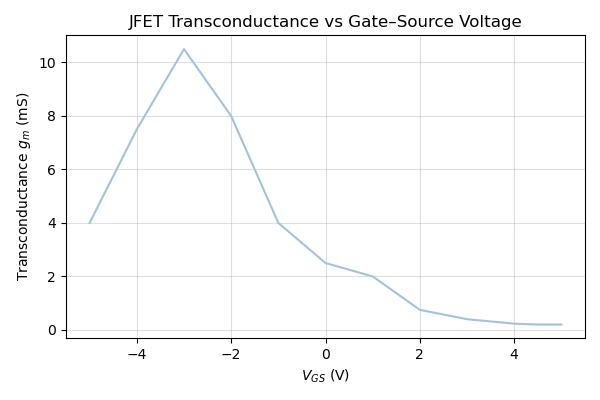
\includegraphics[width=0.8\linewidth]{6.1b.png}
    \caption{Plot of $g_m$ vs. $V_{GS}$ for the J112 n-channel JFET.}
    \label{fig:jfet_gm}
\end{figure}

\noindent The transconductance increases as the gate-source voltage becomes less
negative, reaching a maximum of a little over $10\si{\milli\siemens}$ around
$V_{GS}\approx-2.5\si{\volt}$, and then decreases toward zero for positive 
gate voltages. Our result was within the same order of typical maximum
transconductances for the JFET, and the curve aligned with the general expected behavior.


\subsection{N-channel MOSFET properties}

\subsubsection{Drain current vs. Gate-source voltage}

In this section, observed characteristics of the 2N7000 n-channel MOSFET by
measuring the drain current $I_D$ as a function of the gate-source voltage $V_{GS}$
from $0\si{\volt}$ to approximately $6\si{\volt}$ while keeping the drain 
supply voltage fixed at $10\si{\volt}$ with a $50\si{\ohm}$ series resistor
to limit current. Figure~\ref{fig:mosfet_id_vgs} shows the transistor's threshold 
and saturation behavior.

\begin{figure}[H]
    \centering
    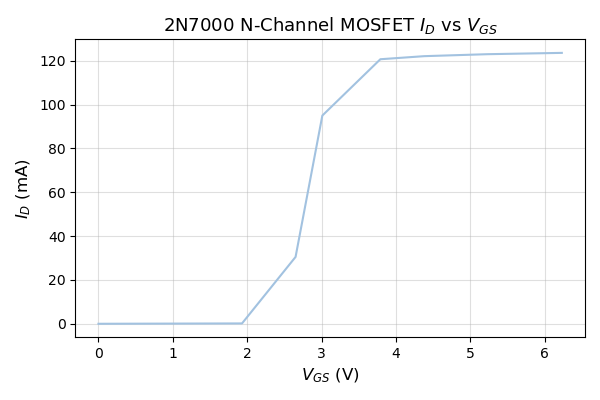
\includegraphics[width=0.8\linewidth]{6.2a.png}
    \caption{Plot of $I_D$ vs.\ $V_{GS}$ for the 2N7000 n-channel MOSFET.}
    \label{fig:mosfet_id_vgs}
\end{figure}

\noindent From the curve above, we observed that the drain current remains near
zero until $V_{GS}$ exceeds the threshold voltage at $V_{GS,th}\approx2\si{\volt}$, 
after which it increases rapidly and saturates around $120\si{\milli\ampere}$ for
$V_{GS} > 3.5\si{\volt}$.\\

\noindent From our observed data, the drain current of $I_D\approx100\si{\milli\ampere}$ occurred at
approximately $V_{GS}=3.1\si{\volt}$, which makes the increment in gate voltage:
\begin{equation}
    \Delta V = V_{GS}-V_{GS,th}=3.1-2.0=1.1\si{\volt}.
\end{equation}

\noindent At $V_{GS}=5.23\si{\volt}$, the measured drain current was
approximately $123\si{\milli\ampere}$. With a $10\si{\volt}$ supply and a $50\si{\ohm}$
resistor in series with the drain, we calculated the drain-source voltage $V_{DS}$ as:

\begin{equation}
    V_{DS}=V_{DD}-I_D R_D=10-(0.123\si{\ampere})(50\si{\ohm})=3.85\si{\volt}.
\end{equation}

\noindent Thus, the corresponding on-resistance of the MOSFET is:
\begin{equation}
    R_{DS(\text{on})}=\frac{V_{DS}}{I_D}=\frac{3.85}{0.123}\approx31.3\si{\ohm}.
\end{equation}

\noindent We also calculated the transconductance $g_m=\frac{\Delta I_D}{\Delta V_{GS}}$. 
The resulting plot in Figure~\ref{fig:mosfet_gm} shows that $g_m$ rises sharply near
the threshold region and peaks around $V_{GS}\approx3\si{\volt}$ at a maximum
of about $130\si{\milli\siemens}$, and then decreases as the MOSFET enters the
saturation region. This behavior agrees with the expected characteristics of the
2N7000.

\begin{figure}[H]
    \centering
    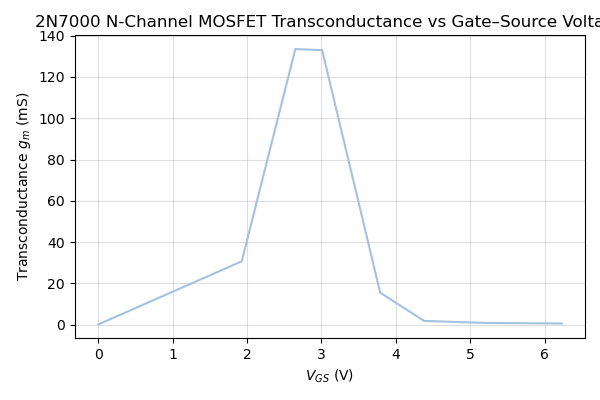
\includegraphics[width=0.8\linewidth]{6.2b.png}
    \caption{Plot of $g_m$ vs.\ $V_{GS}$ for the 2N7000 n-channel MOSFET.}
    \label{fig:mosfet_gm}
\end{figure}


\subsubsection{Drain current vs. Drain-source voltage}

In this section, we measured drain current $I_D$ as a function of the
drain-source voltage $V_{DS}$ for the 2N7000 n-channel MOSFET while keeping
the gate-source voltage fixed at $V_{GS}=5\si{\volt}$. The resulting plot
in Figure~\ref{fig:mosfet_id_vds} shows the expected MOSFET behavior. The
drain current increases approximately linearly for $V_{DS}$ in the ohmic
region, then levels off into saturation around $I_D\approx120\si{\milli\ampere}$
for $V_{DS} > 2\si{\volt}$.

\begin{figure}[H]
    \centering
    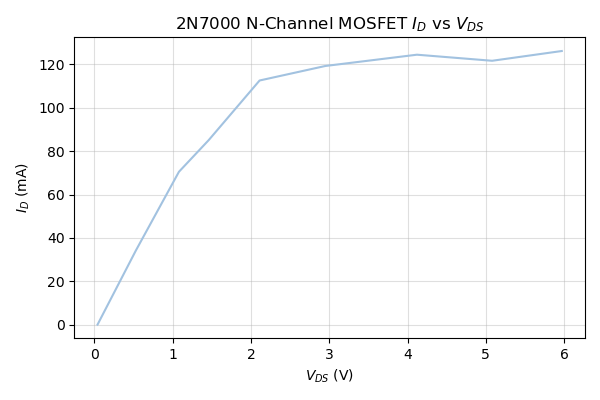
\includegraphics[width=0.8\linewidth]{6.2c.png}
    \caption{Plot of $I_D$ vs.\ $V_{DS}$ for the 2N7000 n-channel MOSFET at $V_{GS} = 5$V.}
    \label{fig:mosfet_id_vds}
\end{figure}

\noindent To estimate the MOSFET's channel resistance in the linear (ohmic) 
region, we selected two data points from the $I_D$ vs.\ $V_{DS}$ curve
where the transistor operates below saturation. Using Ohm’s law:

\begin{equation}
    R = \frac{\Delta V_{DS}}{\Delta I_D} = \frac{1.08 - 0.53}{(70.5 - 34.2) \times 10^{-3}} \approx \frac{0.55}{0.0363} \approx 15.2\si{\ohm}.
\end{equation}

\noindent This calculated resistance represents the MOSFET’s on-state channel resistance
$R_{DS(\text{on})}$ at $V_{GS} = 5\,\si{\volt}$. While this is somewhat higher than the typical 
$R_{DS(\text{on})}$ values listed in the datasheet for similar $V_{GS}$ and $I_D$ conditions, the discrepancy can be attributed to measurement conditions, 
contact resistance, and the fact that our operating current was below the device’s rated maximum.

\subsection{Power MOSFET switching of a load}

Finally, we built the circuit from Fig. VI-3(a) to observe how a power
MOSFET controls current through a resistive load, which in this case is a lamp.
With the MOSFET turned on, we recorded the following measurements:

\begin{enumerate}
    \item Lamp current: $I_{\text{lamp}}=1.192\si{\ampere}$
    \item Voltage across lamp: $V_{\text{lamp}}=4.37\si{\volt}$
    \item Voltage across MOSFET (drain-to-source): $V_{DS}=0.90\si{\volt}$
\end{enumerate}

\noindent To calculate the on-state resistance of the MOSFET, we used Ohm's law:
\begin{equation}
    R_{DS(\text{on})}=\frac{V_{DS}}{I_{\text{lamp}}}=\frac{0.90}{1.192}\approx0.755\si{\ohm}
\end{equation}

\noindent According to the datasheet, the typical value of $R_{DS(\text{on})}$ is 
$0.54\si{\ohm}$ at $V_{GS} = 5\si{\volt}$ and $I_D = 3.4\,\si{\ampere}$, 
with a maximum specified value of $0.76\si{\ohm}$. Our measured resistance of 
$0.755\si{\ohm}$ is slightly above the typical value but within the 
expected range considering differences in test current and measurement conditions.\\

\noindent The power dissipated in the lamp was:
\begin{equation}
    P_{\text{lamp}} = I_{\text{lamp}} \cdot V_{\text{lamp}} 
    = (1.192)(4.37) \approx 5.21\si{\watt},
\end{equation}
whereas the power dissipated in the MOSFET was:
\begin{equation}
    P_{\text{MOSFET}} = I_{\text{lamp}} \cdot V_{DS} 
    = (1.192)(0.90) \approx 1.07\si{\watt}.
\end{equation}

\noindent The total power delivered to the circuit was:
\begin{equation}
    P_{\text{total}} = P_{\text{lamp}} + P_{\text{MOSFET}} 
    = 5.21 + 1.07 = 6.28\si{\watt}.
\end{equation}
Thus, the fraction of power dissipated in the MOSFET was:
\begin{equation}
    \frac{P_{\text{MOSFET}}}{P_{\text{total}}} 
    = \frac{1.07}{6.28} \approx 17.0\%.
\end{equation}

\noindent When we disconnected the gate from the supply, the lamp remained lit briefly 
before gradually dimming. This occurred because the MOSFET’s gate capacitance retained charge, 
temporarily keeping the transistor in conduction. As the gate voltage slowly discharged through leakage paths, 
the MOSFET eventually turned off and the lamp faded.

\end{document}